%\documentclass[english,10pt, compress]{beamer}
\documentclass[english,10pt, compress, handout]{beamer}
\usepackage{mathptmx}
\usepackage[T1]{fontenc}
\usepackage[latin9]{inputenc}
\usepackage{color}
\usepackage{array}
\usepackage{multirow}
\usepackage{amsmath}
\usepackage{amssymb}
\usepackage{fancyvrb}
\makeatletter

%%%%%%%%%%%%%%%%%%%%%%%%%%%%%% LyX specific LaTeX commands.
\newcommand{\noun}[1]{\textsc{#1}}
%% Because html converters don't know tabularnewline
\providecommand{\tabularnewline}{\\}

%%%%%%%%%%%%%%%%%%%%%%%%%%%%%% Textclass specific LaTeX commands.
 % this default might be overridden by plain title style
 \newcommand\makebeamertitle{\frame{\maketitle}}%
 \AtBeginDocument{
   \let\origtableofcontents=\tableofcontents
   \def\tableofcontents{\@ifnextchar[{\origtableofcontents}{\gobbletableofcontents}}
   \def\gobbletableofcontents#1{\origtableofcontents}
 }
 \long\def\lyxframe#1{\@lyxframe#1\@lyxframestop}%
 \def\@lyxframe{\@ifnextchar<{\@@lyxframe}{\@@lyxframe<*>}}%
 \def\@@lyxframe<#1>{\@ifnextchar[{\@@@lyxframe<#1>}{\@@@lyxframe<#1>[]}}
 \def\@@@lyxframe<#1>[{\@ifnextchar<{\@@@@@lyxframe<#1>[}{\@@@@lyxframe<#1>[<*>][}}
 \def\@@@@@lyxframe<#1>[#2]{\@ifnextchar[{\@@@@lyxframe<#1>[#2]}{\@@@@lyxframe<#1>[#2][]}}
 \long\def\@@@@lyxframe<#1>[#2][#3]#4\@lyxframestop#5\lyxframeend{%
   \frame<#1>[#2][#3]{\frametitle{#4}#5}}
 \newenvironment{topcolumns}{\begin{columns}[t]}{\end{columns}}
 \def\lyxframeend{} % In case there is a superfluous frame end


%\setbeamersize{text margin left=.5cm, text margin right=.5cm, text}
% I personally don't think the navigation symbols add anything useful

\hypersetup{colorlinks, urlcolor=blue, linkcolor=magenta}

\usetheme{Warsaw}

\DeclareRobustCommand{\CC}{\hbox{C\hspace{-0.5ex}
                       \protect\raisebox{0.5ex}
                       {\protect\scalebox{0.67}{++}}}}



\newcommand{\Emph}[1]{\textcolor{magenta}{{#1}}}


\usefonttheme{serif}
%\usefonttheme{stillsanserifsmall}
\setbeamercovered{transparent}

\makeatother

\usepackage{babel}
\begin{document}





\title[\CC11]{Moving to Modern CC}


\subtitle {Smart Pointers}


\author[Dave Steffen]{Dave~Steffen \\
{\tiny with a lot of help
from the C++ Deities.}}


\titlegraphic{
\includegraphics[scale=0.1]{SciTecLogo.jpeg}}

\makebeamertitle


\AtBeginSubsection[]{

  \frame<beamer>{

    \frametitle{Outline}

    \tableofcontents[currentsection,currentsubsection]

  }

}



%\beamerdefaultoverlayspecification{<+->}


\lyxframeend{}\lyxframe{Outline}

\tableofcontents{}




\lyxframeend{}

%%%%%%%%%%%%%%%%%%%%%%%%%%%%%%%%%%%%%%%%%%%%%%%%%%%%%%%%%%%%%%%%%%%%%%
%%%%%%%%%%%%%%%%    SLIDES     %%%%%%%%%%%%%%%%%%%%%%%%%%%%%%%%%%%%%%%
%%%%%%%%%%%%%%%%%%%%%%%%%%%%%%%%%%%%%%%%%%%%%%%%%%%%%%%%%%%%%%%%%%%%%%




\section{Intro}

\section{Intro: \CC11}

\lyxframeend{}\subsection[\CC 11]{{\CC 11} high points}


\begin{frame}[fragile,t]
\frametitle{\CC11 : Major Changes}

\begin{itemize}

  \item \textquotedblleft{}\CC11 feels like a new language.\textquotedblright{} --- Bjarne Stroustrup
    \pause{}

  \item \textasciitilde{}10 features pervasively change \CC\ coding
    syle, idioms, and guidance.
    \pause{}
    {\scriptsize
    \begin{enumerate}
    \item \Emph{nullptr}
    \item \Emph{auto}
    \item \Emph{initializer lists}
    \item \Emph{range-based for loop}
    \item smart pointers
    \item lambdas
    \item move semantics
    \item Class support / extensions
    \item atomic operations / threading
    \item enum class
    \end{enumerate}
}
\end{itemize}

%}
%\end{columns}
\end{frame}

\lyxframeend{}


\begin{frame}[fragile]
\frametitle{\CC11 References}
\framesubtitle{E.G., where Dave stole all this material from}
\begin{itemize}
  \item New books to update style, idioms and guidance:
    \begin{itemize}
    \item \noun{What:} T\CC~PL 4th Ed (Stroustrup) now available

    \item \noun{Why and How}: Style (Meyers) -- ``Effective Modern
      \CC'',  2014.

    \item \noun{Thou Shalt}: \CC\ Coding Standards (Sutter \&
    Alexandrescu, 2005) updated by an extensive website \url{https://isocpp.org/faq}.

    \end{itemize}
\end{itemize}
\end{frame}
%% \lyxframeend{}




%% \begin{frame}[fragile,t]
%% \frametitle{\CC\ Standards through the ages}
%% \begin{description}
%% \item[1985]: First Commerical Release, T\CC~PL, 1st Ed
%% \item[1991]: T\CC~PL, 2nd Ed, added templates and exceptions
%% \item[1997]: T\CC~PL, 3rd Ed, introduced ISO standard, added STL
%% \item[1998]: ISO \CC Standard (``\CC 98'')
%% \item[2003]: \CC 03 (``bug fix'' ISO Standard)\par
%% \item[2007]: TR1 (library additions): shared\_ptr, hash tables
%% \item[2011]: \CC 11, major revisions (what we're talking about today)
%% \item[2013]: Complete \CC11 implementations (GCC 4.8, CLANG 3.2)
%% \item[2014]: \CC 14   ``Bug fix'' to \CC11
%% \item[2017]: \CC17 New stuff; complete implementation in GCC 7
%% \item[2020]: \CC20 (?) In progress
%% \end{description}
%% \end{frame}


%% \lyxframeend{}%\lyxframe{\CC11 : Major Changes}








%% \begin{frame}[fragile]
%% \frametitle{\CC11 References}
%% \framesubtitle{E.G., where Dave stole all this material from}

%% \begin{itemize}
%% \item {\bf The} \CC\ Web Page: {\url{http://isocpp.org}}.  Has links to the actual standard document, blogs, etc.
%%       \begin{itemize}
%%       \item The FAQ at {\footnotesize \url{https://isocpp.org/faq}} has a section devoted to \CC11 features.
%%       \end{itemize}
%% \item GoingNative12 and 13: a bunch of \emph{really} good
%%       talks. {\footnotesize \url{http://herbsutter.com/2012/02/08/going-native-sessions-online/}} and
%%       {\footnotesize \url{http://channel9.msdn.com/Events/GoingNative/2013}}
%% \item CppCon (took over for GoingNative in 2014) talks on YouTube.
%% \item Stroustrup's home page and FAQ. {\footnotesize \url{http://www2.research.att.com/~bs}}
%% \item Herb Sutter's Blog and GOTW {\footnotesize \url{http://herbsutter.com/}}
%% \item C++ Next, particularly Dave Abrahams' discusson of move
%% semantics: {\footnotesize \url{http://web.archive.org/web/20140113221447/http://cpp-next.com/archive/2009/08/want-speed-pass-by-value/}}


%% \item GCC \CC11/14/17 support: {\footnotesize \url{https://gcc.gnu.org/projects/cxx-status.html}}


%% \end{itemize}


%% \end{frame}



%% \begin{frame}[fragile]
%% \frametitle{The rest of this talk}
%% \framesubtitle{``Hitting the high points''}

%% \begin{itemize}

%%         \item auto
%%         \item uniform initialization / initializer lists
%%         \item range-based for loops
%%         \item nullptr
%% %        \item Class extensions
%% %        \item lambdas (and sermon on standard containers and algorithms)
%% %        \item move semantics
%% %        \item smart pointers (and sermon on RAII, SESE, etc)
%% \end{itemize}

%% \end{frame}


\section[The Problem]{Memory Management Is The Problem}

\begin{frame}[fragile,t]
\frametitle{Dynamic Memory Is Hard}
\framesubtitle{``If you write C-style code, you expect to have C-style problems'' -- Stroustrup}

{\scriptsize \begin{verbatim}
void foo() {
  double* d = new double[70];
  ...
  if (condition1)
    return;       // Leak!
  ...
  if (error)
    throw ex;     // Leak!

  foo()           // if an exception happens
                  // in here -- Leak!

  delete d;      // cleanup (?)
}
\end{verbatim}}
\end{frame}




%%%%%%%%%%%%%%%%%%%%%%%%%%%%%%%%%%%%%%%%%%%%%%%%%%%%%%%%%%%%%%%%%%%%%%
\begin{frame}[fragile,t]
\frametitle{SESE}

Single-Entry-Single-Exit is an attempt to mitigate this problem:

\begin{columns}[t]
\column{.5\textwidth}
Heavily nested if-blocks:
{\scriptsize\begin{verbatim}
void foo() {
  if (precondition1) {
    double* d = new double[70];
    if (d) {
      ...
      if (precondition2) {
        Widget* w = new Widget;
        if (w) {
           // finally do some work
           FiddleWidget(w);
           ...
           }
        delete w;
        }
     }
   delete d[];
   }
  return;
}
\end{verbatim}}
\pause{}
\column{.5\textwidth}
And doesn't help anyway
{\scriptsize\begin{verbatim}


// Can throw in C++11



// ... might throw



// might throw






\end{verbatim}}
\end{columns}
\pause{}
In the presence of exceptions, \Emph{every function call} can exit the function
\end{frame}


%%%%%%%%%%%%%%%%%%%%%%%%%%%%%%%%%%%%%%%%%%%%%%%%%%%%%%%%%%%%%%%%%%%%%%

\begin{frame}[fragile,t]
\frametitle{Exceptions Break Things}
\framesubtitle{If you don't know what you're doing}
In the presence of exceptions, writing code the old way is nearly impossible:
{\scriptsize\
\begin{verbatim}
void foo() {
  try {  double* d = new double[70]; }
  catch (...) {...}
  ...
  try { foo(); }
  catch (...) { delete d; ...}

  try { bar(); } 
  catch (...) { delete d; ...}

  delete d;      // cleanup
}
\end{verbatim}
}
Every statement must be wrapped in a try/catch block... this is part of the reason exceptions have a bad rap in C++.
\end{frame}

%%%%%%%%%%%%%%%%%%%%%%%%%%%%%%%%%%%%%%%%%%%%%%%%%%%%%%%%%%%%%%%%%%%%%%

\begin{frame}[fragile,t]
\frametitle{}
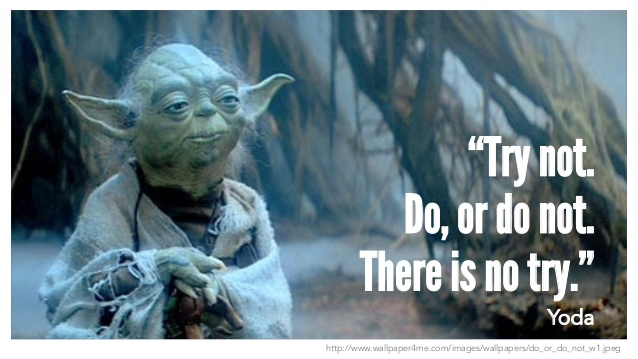
\includegraphics[scale=0.5]{yoda.jpg}

Many (most?) C++ code bases \emph{do not use exceptions}, including
Google's, and including ours.

Writing code \emph{as if} in the presence of exceptions makes code better.

\end{frame}

\begin{frame}[fragile,t]
\frametitle{A Rant}
\framesubtitle{Before we go on...}
There is something very wrong here:
\pause{}
{\scriptsize \begin{verbatim}
void foo() {

  Widget* w = new Widget;
  ...
  if (condition1)
    return;       // Leak!
  ...
  if (error)
    throw ex;     // Leak!

  foo()           // an exception happens
                  // in here -- Leak!

  delete w;      // cleanup 
}
\end{verbatim}}
\pause
\Emph{This isn't Java, so stop it.}

\end{frame}

\begin{frame}[fragile,t]
\frametitle{A Rant}
\framesubtitle{Before we go on...}
Don't hit the heap if you don't have to!

{\scriptsize \begin{verbatim}
void foo() {

  Widget w;      // On the stack!
  ...
  if (condition1)
    return;       // nothing to leak
  ...
  if (error)
    throw ex;     // no problems

  foo()           // an exception happens in here... ok
}
\end{verbatim}}
\pause{}
\begin{itemize}
\item Save runtime
\item Reduce pressure on the heap
\item Reduce memory fragmentation
\pause{}
\item \Emph{Repent, ye Java programmers}
\end{itemize}

\end{frame}

%%%%%%%%%%%%%%%%%%%%%%%%%%%%%%%%%%%%%%%%%%%%%%%%%%%%%%%%%%%%%%%%%%%%%%%%%%%%%%%%

\begin{frame}[fragile,t]
\frametitle{Why dynamic memory at all?}
\center{When must we hit the heap?}
\vskip 6pt
\pause{}

\begin{enumerate}
\item We don't know how many we need until runtime
{\scriptsize \begin{verbatim}
int n;
cin >> n;
Widget* widgets = new Widget[n];
\end{verbatim}
}
\pause{}
\item We don't know what type we need until runtime (polymorphism)
{\scriptsize \begin{verbatim}
class DooDad : public Widget {};
class DooHickey : public DooDad {};
class Gadget : public Widget{}
class Thingy : public Gadget{};

Widget* widget = WidgetFactory(...);
\end{verbatim}
}
\pause{}
\item We don't know how long it's going to live (special case of \#1)
\end{enumerate}

\vskip 12pt
\pause{}

\center{ \Emph{Dynamically allocate only when absolutely necessary} }
\end{frame}


\section[The Solution]{The Solution: RAII}
%%%%%%%%%%%%%%%%%%%%%%%%%%%%%%%%%%%%%%%%%%%%%%%%%%%%%%%%%%%%%%%%%%%%%%
\begin{frame}[fragile,t]
\frametitle{RAII}
\framesubtitle{Resource Aquisition Is Initialization}
\begin{itemize}
\item Smart pointers are a specific case of a more general idiom, ``RAII''
\item Developed to manage resources in the presence of exceptions, but
  they are much more widely useful.
\item The key idea:  \Emph{Tie resource management to object lifetime}
\item Resource manager objects receive the resource in their
  ctor, and release it in their dtor.  Emphasis:
\begin{itemize}
  \item Allocate resource in constructor (at initialization)
  \item Release resources in destructor (at scope exit)
\end{itemize}
\item Normal scoping rules now ensure proper cleanup.
\item Exceptions cause local variables to be destructed, so no leaks.
\end{itemize}
\vskip 12pt
\pause{}
\center{\Emph{ The most important operation in \CC: }}
\pause{}
\center{\Emph{\texttt{\}}}}

\end{frame}


%%%%%%%%%%%%%%%%%%%%%%%%%%%%%%%%%%%%%%%%%%%%%%%%%%%%%%%%%%%%%%%%%%%%%%
\begin{frame}[fragile,t]
\frametitle{Dynamic Memory Is Easy}
{\scriptsize\
\begin{verbatim}
OLD:                              NEW:

void foo() {                      void foo() {
  Widget* d = new Widget();          smart_ptr<Widget> d = new Widget();
  ...                                ....
  if (condition1)                    if (condition1) 
    return;       // Leak!             return;        // no leak!
  ...
  if (error)                         if (error)
    throw ex;                          throw ex;      // no leak!
  ...                                ...
  foo(); // throws, leak!            foo();           // no leak!
  ...             

  delete d;      // cleanup          // no delete, no leak!
}                                 } 
\end{verbatim}
}

(for some definition of ``smart\_ptr'')

The smart pointer object receives a dynamically allocated object in
its ctor, and releases it in the dtor, which executes at scope exit.
\end{frame}

%%%%%%%%%%%%%%%%%%%%%%%%%%%%%%%%%%%%%%%%%%%%%%%%%%%%%%%%%%%%%%%%%%%%%%
%%%%%%%%%%%%%%%%%%%%%%%%%%%%%%%%%%%%%%%%%%%%%%%%%%%%%%%%%%%%%%%%%%%%%%
\begin{frame}[fragile,t]
\frametitle{And the code gets cleaner too}

Remember our Single-Entry-Single-Exit example:

\begin{columns}[t]
\column{.5\textwidth}
Heavily nested if-blocks:
{\scriptsize\begin{verbatim}
void foo() {
  if (precondition1) {
    double* d = new double[70];
    if (d) {
      if (conditionA) {
        Widget* w = new Widget;
        if (conditionB) {
           // finally do some work
           ...
           FiddleWidget(w);
           ...
           }
        delete w;
        }
     delete d[];
     }
   }
  return;
}
\end{verbatim}}
\pause{}
\column{.5\textwidth}
Becomes this:
{\scriptsize\begin{verbatim}
void foo() {
  if (!precondition1)  return;
  std::vector<double> d (70); // #1
                              // #2
  if (!precondition2) return;
  smart_ptr<Widget> w = new Widget;
  if (conditionB) return;
  // finally do some work
  ...
  FiddleWidget(w);
  ...






  return;
}
\end{verbatim}}
\end{columns}
\pause{}
\Emph{Even in the absence of exceptions, exception-safe code is cleaner,
faster, and more maintainable.}
\end{frame}


\section[Standard Smart Pointers]{Standard Smart Pointers}
\begin{frame}[fragile,t]
\frametitle{Standard Smart Pointers}
\begin{description}
\vskip 12pt
\item [std::auto\_ptr]  \textcolor{red}{DEPRECATED}
\vskip 12pt
\item [std::unique\_ptr] Single Ownership
\vskip 12pt
\item [std::shared\_ptr] Shared Ownership
\vskip 12pt
\item [std::weak\_ptr] Breaks ownership cycles
\vskip 24pt
\item [std::vector] 
\item [std::set]     Pointers so smart you don't even notice they are (!)
\item [std::map]
\item [...]
\end{description}
\end{frame}


\subsection{auto\_ptr}

\begin{frame}[fragile,t]
\frametitle{auto\_ptr}
An early attempt to provide single ownership semantics.  Copying
transfers ownership.
{\scriptsize\
\begin{verbatim}

auto_ptr<int> a = new int(5);

auto_ptr<int> b = nullptr;

b = a;        // changes a!

a == nullptr; // now true!

\end{verbatim}}

\begin{itemize}
\item Destructive copy! Wonky semantics -- can't use in standard containers, doesn't act
  like anything we have a good model for.
\item (Non-value semantics are always wonky -- avoid)
\item Desired behavior impossible without C++11 move semantics
\end{itemize}
\vskip 12pt
\pause{}
\center{\Emph{Don't Use}}

\end{frame}


%%%%%%%%%%%%%%%%%%%%%%%%%%%%%%%%%%%%%%%%%%%%%%%%%%%%%%%%%%%%%%%%%%%%%%
\subsection{unique\_ptr}


\begin{frame}[fragile]
\frametitle{unique\_ptr}

With the advent of move semantics, we now have a proper solution.

\center{\Emph{std::unique\_ptr}}

\begin{itemize}
\item Provides \Emph{single ownership} of the pointer it holds.
\item Takes ownership on construction
\item \texttt{delete}s the pointer on destruction
\item Provides pointer-like syntax in all cases
\begin{itemize}
  \item initialize with dynamically allocated object
  \item Deref with \texttt{*} and \texttt{->}
  \item Explicit conversion to bool
  \item Can compare to nullptr
\end{itemize}
\item Moveable but non-copyable
\begin{itemize}
  \item Non-copyable: maintains single ownership
  \item Moveable: explicit ownership transfer
\end{itemize}
\item Little or no memory or runtime overhead compared to a raw pointer.
\end{itemize}

\end{frame}

%% %%%%%%%%%%%%%%%%%%%%%%%%%%%%%%%%%%%%%%%%%%%%%%%%%%%%%%%%%%%%%%%%%%%%%%
%% %%%%%%%%%%%%%%%%%%%%%%%%%%%%%%%%%%%%%%%%%%%%%%%%%%%%%%%%%%%%%%%%%%%%%%

\begin{frame}[fragile]
\frametitle{unique\_ptr basics}

\begin{itemize}
\item Use like a pointer
{\scriptsize\begin{verbatim}
#include <memory>

unique_ptr<int> i {new int(4)};
cout << "i " << *i << endl;     // Use just like normal pointer

\end{verbatim}}
\item Moveable, but not copyable
{\scriptsize\begin{verbatim}

unique_ptr<int> j;

j = i;                          // compile error (use of deleted fn)

j = std::move(i);               // OK, *j == 4

assert (i == nullptr);          // true

\end{verbatim}}
\item Moved-from unique\_ptr is null, treat like all moved-from
  objects: \Emph{with care!}  
\end{itemize}

\end{frame}

%%%%%%%%%%%%%%%%%%%%%%%%%%%%%%%%%%%%%%%%%%%%%%%%%%%%%%%%%%%%%%%%%%%%%%

\begin{frame}[fragile]
\frametitle{unique\_ptr other operations}

\begin{itemize}
\item \texttt{get} gets a non-owning copy of the pointer
{\scriptsize\begin{verbatim}
int* nonowner = j.get()         // get the pointer, keep ownership

\end{verbatim}}
\item \texttt{release} return gets an \emph{owning} pointer, and
  relinquishes ownership

{\scriptsize\begin{verbatim}
int* nonowner = j.get()         // get the pointer, keep ownership
int* owner = j.release();       // release ownership, now j==nullptr

j = owner;                      // retake ownership of existing ptr

j.reset();                      // delete ptr, now j==nullptr
\end{verbatim}}
\end{itemize}
\vskip 6pt
\texttt{unique\_ptr} provides the safest (and most restrictive) ownership model.  Prefer
\texttt{unique\_ptr} when possible.

\end{frame}

%%%%%%%%%%%%%%%%%%%%%%%%%%%%%%%%%%%%%%%%%%%%%%%%%%%%%%%%%%%%%%%%%%%%%%%%%%%%%%%%

\begin{frame}[fragile]
\frametitle{Using unique\_ptr}
Given existing code:
{\scriptsize\begin{verbatim}
void ViewWidget    ( const Widget&       );
void FiddleWidget  (       Widget&       );
void ViewWidgetPtr (       Widget* const );
void MungeWidgetPtr(       Widget*       );
\end{verbatim}
}

and a unique\_ptr<Widget> wptr : 

{\scriptsize\begin{verbatim}
ViewWidget     (*wptr);    // pass by const&

FiddleWidget   (*wptr);  // Fine -- change the object, wptr retains owernship

ViewWidgetPtr  (wptr.get()); // OK, the pointer is const

MungeWidgetPtr (wptr.get());  // Danger?
\end{verbatim}}
\begin{itemize}
\item Be careful when passing the pointer to legacy functions -- make sure
they're not taking ownership.
\item If they do, send wptr.release()  (explicitly give up ownership)
\pause{}
\item \Emph{If you're not sure... you have a problem}
\end{itemize}

\end{frame}

%%%%%%%%%%%%%%%%%%%%%%%%%%%%%%%%%%%%%%%%%%%%%%%%%%%%%%%%%%%%%%%%%%%%%%%%%%%%%%%%

% herb sutter, 12:12 - 21:50

\begin{frame}[fragile]
\frametitle{unique\_ptr as function argument}
\framesubtitle{Herb Sutter, GotW \#91}
What do these mean?
{\scriptsize\begin{verbatim}
void f( widget& );                    (a)    f(*wptr)

void f( widget* );                    (b)    f( wptr.get())
                                          or f( wptr.release())
\end{verbatim}}
\begin{itemize}
\pause{}
\item (a) is preferred -- observe or process the object directly
\pause{}
\item (b) is either
\begin{itemize}
  \item Legacy or OS (C code in system library).
  \item Observing or processing \emph{the pointer} (taking ownership,
    reseating, etc), possibly a sink: f is a function that consumes
    pointer-to-widgets and takes ownership of the pointer
  \item Using the NULL ptr as a sentinel value, or the value is optional
  \item Incorrect (Repent ye C programmers!)
\end{itemize}
\end{itemize}
Be careful with C-style (raw pointer) interfaces, the ownership of the
pointer might not be clear, and many times all you have is a comment somewhere:
{\scriptsize\begin{verbatim}
void scary_widget_sink( widget* p); // will destroy p. PLEASE READ THIS
\end{verbatim}}
\end{frame}

%%%%%%%%%%%%%%%%%%%%%%%%%%%%%%%%%%%%%%%%%%%%%%%%%%%%%%%%%%%%%%%%%%%%%%%%%%%%%%%%

%%%%%%%%%%%%%%%%%%%%%%%%%%%%%%%%%%%%%%%%%%%%%%%%%%%%%%%%%%%%%%%%%%%%%%%%%%%%%%%%

% herb sutter, 12:12 - 21:50

\begin{frame}[fragile]
\frametitle{unique\_ptr as function argument (the plot thickens)}
\framesubtitle{Herb Sutter, GotW \#91}

What do these mean?

{\scriptsize\begin{verbatim}
void f (unique_ptr<widget> );         (c)    f( wptr) error!
void f( unique_ptr<widget>&&);        (d)    f( std::move(wptr))
void f( unique_ptr<widget>& );        (e)    f( wptr)
void f( const unique_ptr<widget>& );  (f)    f( wptr)
\end{verbatim}}

\begin{itemize}
\item (c) is a compile-time error -- you can't pass a unique\_ptr by
  value because you can't make copies.
\item (d) is also a sink:  f is a unique\_ptr-to-widget-consuming
  function, wptr becomes null.
\pause{}
\item (e) is for reseating an existing unique\_ptr (when you get it
  back, it might be pointing to something else)
\pause{}
\item (f) is a mistake; there's never any reason to do this.  If
  you're not participating in an ownership transaction, just observe
  the object as per (a).
\end{itemize}

\end{frame}

%%%%%%%%%%%%%%%%%%%%%%%%%%%%%%%%%%%%%%%%%%%%%%%%%%%%%%%%%%%%%%%%%%%%%%%%%%%%%%%%
%% \begin{frame}[fragile]
%% \frametitle{std::make\_unique}
%% \framesubtitle{Item 21, ``Modern Effective C++'' by Scott Meyers}
%% Even better: prefer to initialize \texttt{unique\_ptr}s via
%% \texttt{make\_unique}:
%% {\scriptsize\begin{verbatim}
%% std::unique_ptr<Camel> p {new Camel              (humps, legs, attitude)}; // good
%% std::unique_ptr<Camel> p {std::make_unique<Camel>(humps, legs, attitude)}; // better
%% auto                   p {std::make_unique<Camel>(humps, legs, attitude)}; // best
%% \end{verbatim}}
%% \begin{itemize}
%%   \item Don't repeat the type name
%%   \item Can be more efficient
%%   \item Better exception safety (for arcane reasons)
%%   \item We no longer type 'delete', so we shouldn't type 'new'
%%     \begin{itemize}
%%       \item This is the birth of a new, universally accepted
%%         guideline: \Emph{application code should contain no 'new' or
%%         'delete' keywords, except when writing RAII classes.}
%%     \end{itemize}
%% \end{itemize}

%% Alas, \texttt{make\_unique} was omitted from the \CC11 standard (they
%% just forgot), so it's technically only available in \CC14.  However,
%% you write it yourself:

%% {\scriptsize\begin{verbatim}
%% template<typename T, typename.... Ts>
%% std::unique_ptr<T> make_unique(Ts&&... params) {
%% return std::unique_ptr<T>(new T(std::forward<Ts>(params)...));
%% }
%% \end{verbatim}}
%% ... or use Abseil \url{https://abseil.io/} which will be availble on SOFA.
%% \end{frame}


%%%%%%%%%%%%%%%%%%%%%%%%%%%%%%%%%%%%%%%%%%%%%%%%%%%%%%%%%%%%%%%%%%%%%%%%%%%%%%%%


\begin{frame}[fragile]
\frametitle{unique\_ptr custom deleter}
Custom deleter: provide a function to call for deletion
{\scriptsize\begin{verbatim}
auto dtor = [](int* p) { cout << "Ptr holds " << *p << endl; delete p; };

unique_ptr<int, decltype(dtor)> q {new int(42), dtor};

q.reset();  // prints ``Ptr holds 42''
\end{verbatim}}


\vskip 12pt

More generally, this allows us to run \emph{arbitrary code} when the
object is deleted.

\vskip 6pt
Alas, \texttt{make\_unique} doesn't support this, which is too bad.  We could write a \texttt{allocate\_unique} to do this if desired.

\end{frame}


%%%%%%%%%%%%%%%%%%%%%%%%%%%%%%%%%%%%%%%%%%%%%%%%%%%%%%%%%%%%%%%%%%%%%%%%%%%%%%%%
%%%%%%%%%%%%%%%%%%%%%%%%%%%%%%%%%%%%%%%%%%%%%%%%%%%%%%%%%%%%%%%%%%%%%%%%%%%%%%%%

\subsection{shared\_ptr}

%%%%%%%%%%%%%%%%%%%%%%%%%%%%%%%%%%%%%%%%%%%%%%%%%%%%%%%%%%%%%%%%%%%%%%%%%%%%%%%%
%%%%%%%%%%%%%%%%%%%%%%%%%%%%%%%%%%%%%%%%%%%%%%%%%%%%%%%%%%%%%%%%%%%%%%%%%%%%%%%%

\begin{frame}[fragile]
\frametitle{shared\_ptr}
\Emph{std::shared\_ptr} provides a more common model of ownership
(similar to Python and Java, but with better performance).

\begin{itemize}
\item Shared ownership -- make copies and send 'em out into the big wide
world.

\item Reference counted -- memory released only when the last observer
goes out of scope.

\item Provides the C++ equivalent of a garbage collector, with
  deterministic behavior.

\end{itemize}

{\scriptsize\begin{verbatim}
void foo() 
{  
  shared_ptr<int> p1{new int}; // count is 1
  {
    shared_ptr<int> p2{p1};    // count is 2
    {
      shared_ptr<int> p3{p1};  // count is 3
    }                          // count goes back down to 2
  }                            // count goes back down to 1
}            // here the count goes to 0 and the int is deleted.
\end{verbatim}}

\end{frame}


%%%%%%%%%%%%%%%%%%%%%%%%%%%%%%%%%%%%%%%%%%%%%%%%%%%%%%%%%%%%%%%%%%%%%%

\begin{frame}[fragile]
\frametitle{shared\_ptr part 2}

Other operations:
{\scriptsize\begin{verbatim}

int* p = p1.get();             // get raw pointer (non-owning!!!)

long int use = p1.use_count(); // refcount

bool u = p1.unique();          // true if refcount==1

p1.reset();                    // drops refcount by 1, calls dtor if 0
\end{verbatim}
}



\begin{itemize}
\pause{}
\item Minimal overhead (no more than necessary)
\begin{itemize}
  \item each object has an additional dynamically allocated address to
    store the refcount
  \item Increment/decrement is thread-safe, which means a mutex
\end{itemize}
\vskip 6pt
\pause{}
\item Minimal, but not zero; these have an unjustified bad 
  reputation for bad runtime performance.
\vskip 6pt
\pause{}
\item Beware of circular references (see \texttt{weak\_ptr} discussion below)
\end{itemize}
\end{frame}

%%%%%%%%%%%%%%%%%%%%%%%%%%%%%%%%%%%%%%%%%%%%%%%%%%%%%%%%%%%%%%%%%%%%%%%%%%%%%%%%

\begin{frame}[fragile]
\frametitle{shared\_ptr as function argument}
\framesubtitle{Herb Sutter, GotW \#91}
What do these mean?
{\scriptsize\begin{verbatim}
void f(       shared_ptr<widget> );   (g)
void f(       shared_ptr<widget>& );  (h)
void f( const shared_ptr<widget>& );  (i)
\end{verbatim}
}
\begin{itemize}
\pause{}
\item (g) participates in shared ownership (it's taking a copy, and that's what
  copying a shared\_ptr means)
\pause{}
\item (h) manipulates the shared\_ptr; possibly reseating \emph{this}
  one.  Not commonly used, I couldn't find many good examples.
\pause{}
\item (i) Very uncommon, probably a mistake.  Possibly this means f \emph{might} make a copy?
\end{itemize}
\vskip 12pt
\pause{}
Remember, if you're interested in just the widget, \Emph{take just the widget}.


\end{frame}

%%%%%%%%%%%%%%%%%%%%%%%%%%%%%%%%%%%%%%%%%%%%%%%%%%%%%%%%%%%%%%%%%%%%%%%%%%%%%%%%
\subsection{make\_shared, make\_unique}
\begin{frame}[fragile]
\frametitle{``make'' functions}
\begin{columns}[t]
\column{.5\textwidth}
This is OK
{\scriptsize\begin{verbatim}
unique_ptr<Widget> up = new Widget(...);

shared_ptr<Camel> sp = new Camel(...);
\end{verbatim}}
\pause{}
\column{.5\textwidth}
But this is better
{\scriptsize\begin{verbatim}
auto up = make_unique<Widget>(...);

auto sp = make_shared<Camel>(...);
\end{verbatim}}
\end{columns}
\vskip 12pt
\pause{}
\begin{itemize}
\item Only type the type once : ``DRY'' (Don't Repeat Yourself) principle
\vskip 6pt
\item Performance: make\_functions can have memory and runtime advantages
\item Better exception safety in some cases
\vskip 6pt
\item We are all used to being twitchy about new/delete.  
\begin{itemize}
  \item Trained from birth: see a new, look for the delete
  \item \Emph{This is a good survival habit we don't want to weaken.}
  \item With smart pointers, we don't write delete, so don't write new.
  \end{itemize}
\end{itemize}
\pause{}
\center{\Emph{Never write new or delete again}}

\end{frame}

%%%%%%%%%%%%%%%%%%%%%%%%%%%%%%%%%%%%%%%%%%%%%%%%%%%%%%%%%%%%%%%%%%%%%%%%%%%%%%%%
\begin{frame}[fragile]
\frametitle{make functions part 2}

Alas, \texttt{make\_unique} was omitted from the \CC11 standard (they
just forgot), so it's technically only available in \CC14.  However,
you write it yourself:

{\scriptsize\begin{verbatim}
template<typename T, typename.... Ts>
std::unique_ptr<T> make_unique(Ts&&... params) 
{
  return std::unique_ptr<T>(new T(std::forward<Ts>(params)...));
}
\end{verbatim}}
\vskip 12pt
... or use Abseil (\url{https://abseil.io/}) which will be availble on SOFA.
\vskip 12pt

\begin{center}
This is the birth of a new, universally accepted  guideline: 
\vskip 6pt
\Emph{Application code should contain no 'new' or
  'delete' keywords (except when writing RAII classes).}
\end{center}
\end{frame}




%%%%%%%%%%%%%%%%%%%%%%%%%%%%%%%%%%%%%%%%%%%%%%%%%%%%%%%%%%%%%%%%%%%%%%%%%%%%%%%%
\subsection{std::vector}

\begin{frame}[fragile]
\frametitle{std::vector as a smart pointer?}
\framesubtitle{what madness is this?}

\texttt{std::vector} doesn't have a pointer-like interface, but is the
gold standard of RAII-design classes.

\begin{itemize}

\item Consider: \emph{pointers are confusing, complex, and difficult
  to reason about}.  Hiding that complexity behind value semantics is
  a huge win.

\item Growing and shrinking as needed is handled automatically and safely.

\item Control of memory is still provided via clear(), resize(), and
  reserve() functions.

\item Access to the raw C-style array is provided via the data()
  function.
\begin{itemize}
  \item Similar to the smart pointers' \texttt{get} function, this can
    be used (with care) in legacy C-style interfaces.
\end{itemize}
\end{itemize}

\end{frame}

%%%%%%%%%%%%%%%%%%%%%%%%%%%%%%%%%%%%%%%%%%%%%%%%%%%%%%%%%%%%%%%%%%%%%%%%%%%%%%%%
\begin{frame}[fragile]
\frametitle{std::vector to the rescue}
\framesubtitle{no joke}
Straight out of the HEMI code base: old way (left), std::vector (right):
\begin{columns}[t]
\column{.5\textwidth}
{\tiny\begin{verbatim}
const void* ZlibMem::compress( const void* buffer,
                               size_t* msgBytes )
{
  if (!buffer || !msgBytes || (*msgBytes == 0)) {
    LOG( Logger::ERROR, "long error msg" );
    return NULL;
  }
// get size needed for compress buffer and realloc if needed
  size_t sizeNeeded = compressBound( *msgBytes );
  if (sizeNeeded > compressBufferSz_) {
    compressBuffer_ = 
      (Bytef*)realloc( compressBuffer_, sizeNeeded );
    if (compressBuffer_)
      compressBufferSz_ = sizeNeeded;
    else {
      compressBufferSz_ = 0;
      LOG( Logger::ERROR, realloc failed." );
      return NULL;
    }
  }

\end{verbatim}}
\pause{}
\column{.5\textwidth}
{\tiny\begin{verbatim}
const void* ZlibMem::compress(const std::vector<char>& buffer)

{
  if (buffer.empty()) {
    LOG( Logger::ERROR, "long error msg''" );
    return nullptr;
  }

  size_t sizeNeeded = compressBound(buffer.size() );
  try {
    compressBuffer_.resize(sizeNeeded);
  }
  catch (std::bad_alloc) {
     LOG( Logger::ERROR, "realloc failed.." );
     return nullptr;
  }

 // <-- memory leak over there!  Would you have noticed?
 //     ... no leaks over here.

\end{verbatim}}
\end{columns}
\pause{}

When maintaining old code, hunt down and kill C-style raw arrays
\Emph{with prejudice} and replace with \texttt{std::vector} or
\texttt{std::array}!

\end{frame}





%% %%%%%%%%%%%%%%%%%%%%%%%%%%%%%%%%%%%%%%%%%%%%%%%%%%%%%%%%%%%%%%%%%%%%%%
%% \begin{frame}[fragile]
%% \frametitle{Exception-safe function calls}
%% {\scriptsize Herb Sutter, GOTW 102  \hskip 1in   http://herbsutter.com/gotw/\_102/}
%% \begin{itemize}
%% \item  <1-> What can you say about the order of evaluation?
%% \item[]<1-> {\scriptsize\begin{verbatim}int f( expr1, expr2 ) ;\end{verbatim}}
%% \item[]<1-> {\scriptsize\begin{verbatim}i = f( g (expr1), h (expr2) ) ;\end{verbatim}}
%% %% order of evaluation.
%% %%% All args must be evaluated before the function is called
%% %%% Functions don't interleave
%% %%% Function args can be evaluated in an order, including interleaved,
%% %%%    - unless restricted by other rules
%% %%% :: expr 1 and 2 evalued before f, but may be interleaved
%% %%% || expr 1 and expr 2 interleaved, g and h in any order but not interleaved,
%% %%% exprs before g and h
%% \item  <2-> What are the problems with this?
%% \item[]<2-> {\scriptsize\begin{verbatim}int f( T*, U2* ) ;\end{verbatim}}
%% \item[]<2-> {\scriptsize\begin{verbatim}i = f( new T, new U ) ;\end{verbatim}}
%% %% uh-oh.  If exception between memory allocation
%% \item  <3-> Throw smart pointers at the problem -- no dice
%% \item[]<3-> {\scriptsize\begin{verbatim}int f( unique_ptr<T>, unique_ptr<U> ) ;\end{verbatim}}
%% \item[]<3-> {\scriptsize\begin{verbatim}i = f( new T, new U ) ; // just as bad\end{verbatim}}
%% \item[]<3-> {\scriptsize\begin{verbatim}i = f( unique_ptr<T>(new T), unique_ptr<U>(new U) ) ;\end{verbatim}}
%% % No -- no better.  Still separation between memory allocation and initialization
%% \item  <4-> The correct solution
%% \item[]<4-> {\scriptsize\begin{verbatim}i = f( make_unique<T>(), make_unique<U>()) ;\end{verbatim}}
%% %%% OK -- now we're safe within function calls
%% \end{itemize}

%% Bigger point -- we are all used to being twitchy about new/delete.  We
%% see a new, we look for the delete

%% This is a *good survival habit* we don't want to weaken.

%% Smart ptrs... we don't write delete, so don't write new.

%% There are some arcane issues involved.... extra slide.

%% \end{frame}



%%%%%%%%%%%%%%%%%%%%%%%%%%%%%%%%%%%%%%%%%%%%%%%%%%%%%%%%%%%%%%%%%%%%%%%%%%%%%%%%


\subsection{weak\_ptr}
\begin{frame}[fragile]
\frametitle{weak\_ptr}
\framesubtitle{Handle circular shared\_ptrs}

\begin{itemize}
\item Non-owning observer of a shared\_ptr-managed resource
{\scriptsize\begin{verbatim}
shared_ptr<int> a {new int(42)}; // refcount == 1
shared_ptr<int> b {a}            //      now == 2

weak_ptr<int> w {b};             // points to same int,
                                 // leaves refcount at 2
assert (*w == 42);     // error! Can't deref weak ptr
\end{verbatim}
}
\pause{}
\item No deref operator!  This is for your protection, because the
  thing it points to may be gone.
\pause{}
\item To access the thing, lock:
{\scriptsize\begin{verbatim}

shared_ptr<int> c = w.lock();   // convert to shared_ptr, refcount == 3

assert( c );               // ok if the thing still exists

assert (!w.expired());           // another way to check

a.reset();  // refcount == 2
b.reset();  // refcount == 1
c.reset();  // refcount == 0, ptr deleted

assert (w.expired());
shared_ptr<int> bad = w.lock();  // bad == nullptr
\end{verbatim} 
}
\end{itemize}
\end{frame}

\begin{frame}[fragile]
\frametitle{weak\_ptr part 2}
Use for things that may or may not exist
\begin{itemize}
\item If the thing exists, use it (via the shared\_ptr created by locking)
\item If the thing doesn't exist, you can test and do something reasonable.
  \begin{itemize}
  \item \Emph{If there's nothing reasonable, you have a big design problem.}
  \end{itemize}
\end{itemize}
\pause{}
\vskip 12pt
Example from Herb Sutter: factory with cache
{\scriptsize\begin{verbatim}
shared_ptr<widget> make_widget(int id) 
{
  static map<int, weak_ptr<widget>> cache;

  auto sp = cache[id].lock();

  if (!sp) cache[id] = sp = load_widget(id);

  return sp;
}
\end{verbatim}
}

\vskip 12pt
\pause{}

\center{\Emph{Use when necessary (and you'll know when it's necessary)}}

\end{frame}



\section{Summary}
%%%%%%%%%%%%%%%%%%%%%%%%%%%%%%%%%%%%%%%%%%%%%%%%%%%%%%%%%%%%%%%%%%%%%%
\begin{frame}[fragile,t]
\frametitle{Summary}
\begin{itemize}[<+->]
\item \texttt{type\_traits.h} defines more type traits than would be
  wise to shake a stick at
\begin{itemize}
  \item Pay particular attention to \texttt{enable\_if}.
\end{itemize}
\item \cexpr is \emph{the} way to do compile-time value computations.
\begin{itemize}
  \item Prefer over recursive templates in all cases.
\end{itemize}
\item Variadic templates
\begin{itemize}
  \item \Emph{Wow}.  Or \Emph{Ouch}.  Or both.
\end{itemize}
\item Universal References and Perfect Forwarding.
\begin{itemize}
  \item Solutions to problems you didn't know you had (but you'd find
    out the hard way).
\end{itemize}
\end{itemize}
\end{frame}

%%%%%%%%%%%%%%%%%%%%%%%%%%%%%%%%%%%%%%%%%%%%%%%%%%%%%%%%%%%%%%%%%%%%%%
\begin{frame}[fragile,t]
\frametitle{Encouragement}
\begin{itemize}[<+->]
\item \Emph{This stuff is not academic}
\item Fundamental power-tools for library writers.
\item Fundamental power-tools for non-library writers.
\item Jason Turner: \CC17 game code for Commodore
  64. \url{https://www.youtube.com/watch?v=zBkNBP00wJE&t=1488s}
\vskip 6pt
\item A concern shared amongst many people in the Standards Committee:
\begin{itemize}
  \item People aren't thinking compile-time enough.
  \item Compile-time stuff is \emph{everywhere}
  \item Embedded work is \Emph{particularly} receptive / amenable /
    desperate for these techniques.
\end{itemize}
\end{itemize}
\pause
\vskip 24pt
\begin{center}
\Emph {Go Forth And Compile-Time Program!!!}
\end{center}
\end{frame}

%%%%%%%%%%%%%%%%%%%%%%%%%%%%%%%%%%%%%%%%%%%%%%%%%%%%%%%%%%%%%%%%%%%%%%
%% \begin{frame}[fragile,t]
%% \frametitle{}
%% \end{frame}


\end{document}
